\section{Сходимость Q-learning}\label{appendix:qlearning}

В данном разделе приведено доказательство теоремы \ref{th:TDconvergencetheorem}. Пусть дано MDP с конечным пространством состояний $\St$ и действий $\A$. $Q^*_0(s, a)$ --- начальное приближение, на $k$-ом шаге $Q^*_k(s, a)$ строится по правилу
\begin{equation}\label{Qlearningupdateproof}
Q^*_{k+1}(s, a) = (1 - \alpha_k(s, a))Q^*_k(s, a) + \alpha_k(s, a) \left( r(s, a) + \gamma \max_{a'} Q^*_k(s', a')\right)
\end{equation}
где $s' \sim p(s' \mid s, a)$, а $\alpha_k(s, a)$ --- случайные величины, на которые накладывается единственное требование: для всех $s, a$ с вероятностью 1 выполнено:
\begin{equation}\label{TDconvergenceconditionsproof}
\sum_{k \ge 0} \alpha_k(s, a) = +\infty \qquad \sum_{k \ge 0} \alpha_k(s, a)^2 < +\infty
\end{equation}

\subsection{Action Replay Process}

Для доказательства рассмотрим конструкцию под названием Action Replay Process. Давайте запустим алгоритм Q-learning (проведём, чисто теоретически, бесконечное число итераций) и запишем для каждого реализации $\alpha_k(s, a)$ и $s'_k(s, a)$ --- те следующие состояния, которые использовались на $k$-ом шаге для обновления $Q^*_k(s, a)$. Будем проводить такую аналогию --- запишем эту историю <<на карточках>>: на $k$-ой карточке записано для каждой пары $s, a$ по одному сэмплу $s'_k(s, a) \HM\sim p(s' \HM\mid s, a)$, а также степень $\alpha_k(s, a)$, с которой этот сэмпл был использован для обновления Q-функции; можно считать, что для них в случившейся реализации выполнено \eqref{TDconvergenceconditionsproof}, поскольку это происходит с вероятностью 1. Карточки, считаем, <<сложены в стопку>>, начиная с нулевой карточки, на которой, условно, напишем наше исходное приближение Q-функции $Q_0(s, a)$ для всех $s, a$. Мы сейчас будем эту стопку карт <<просматривать>> от конца к началу.

\newcommand{\ARP}{\mathrm{ARP}}
\begin{definition}
Для данной реализации алгоритма Q-learning Action Replay Process (ARP) будем называть следующее MDP:
\begin{itemize}
    \item Пространством состояний будем считать пару $s, n$, где $s \in \St$, $n$ --- номер карточки.
    \item Пространством действий будем считать $\A$.
    \item Процесс генерации следующего состояния по данному состоянию $s, n$ и действию $a$, который мы будем обозначать как $p_{\ARP}(s', n' \mid s, n, a)$, задаётся следующим образом. Если номер карточки $n$ равен нулю, то <<стопка карт закончилась>>, и следующее состояние --- терминальное. Если $n > 0$, то бросаем нечестную монетку, которая с вероятностью $\alpha_{n - 1}(s, a)$ выдаёт результат <<остановиться>>, а с вероятностью $1 \HM- \alpha_{n - 1}(s, a)$ выдаёт результат <<пойти дальше>>. <<Остановиться>> означает, что мы полагаем итоговым следующим состоянием пару $s'_{n - 1}(s, a), n - 1$. <<Пойти дальше>> означает, что верхняя карточка колоды удаляется --- $n$ всё равно уменьшается на единицу, --- и процедура повторяется уже для тройки $s, n - 1, a$: мы снова подбрасываем монетку и так далее, пока не выпадет <<остановиться>> или колода карт не закончится.
    \item Награда для тройки $s, n, a$ есть $r(s, a)$, если $n > 0$, и $Q_0^*(s, a)$ иначе.
\end{itemize}
\end{definition}

\needspace{7\baselineskip}
\begin{wrapfigure}{r}{0.35\textwidth}
\vspace{-0.3cm}
\centering
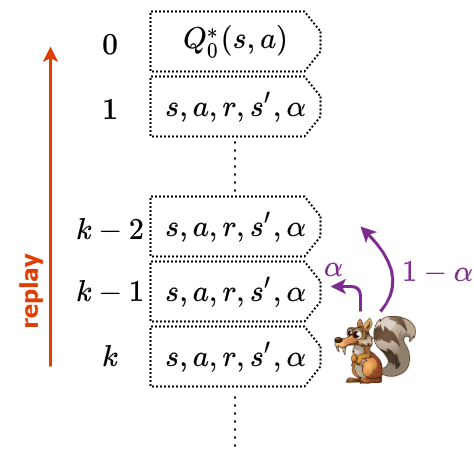
\includegraphics[width=0.35\textwidth]{Images/ARP.png}
%\vspace{-0.3cm}
\end{wrapfigure}

Данное определение внезапно содержит в себе всю основную идею доказательства. Что тут происходит? Давайте посмотрим на первые $n$ шагов результаты работы Q-learning-а. Попробуем построить MDP, которое было бы в некотором смысле <<похожее>> на исходное MDP, но использующее только собранную историю (т.к. доступа к $p(s' \mid s, a)$ у нас нет). Если $n \HM= 0$, и истории нет, то мы считаем, что мы бы получили $Q^*_0(s, a)$ в качестве награды за всю оставшуюся игру --- такого наше <<исходное>> приближение MDP. Для больших $n$ для данной пары состояние-действие мы в качестве следующего состояния хотели бы засэмплировать $s' \HM\sim p(s' \HM\mid s, a)$, но вместо этого у нас есть лишь коллекция $s'_k(s, a)$. Давайте с вероятностью $\alpha_{n-1}(s, a)$ возьмём в качестве сэмпла $s'_n(s, a)$, с вероятностью $(1 \HM- \alpha_{n-1}(s, a))\alpha_{n-2}(s, a)$ возьмём в качестве сэмпла $s'_{n-1}(s, a)$, и так далее. Мы знаем, что при стремлении $n$ к бесконечности альфы, во-первых, уходят к нулю (это гарантирует сходимость ряда из квадратов альф), а во-вторых, сэмплов будет бесконечно много (бесконечно много альф обязано быть ненулевыми из-за расходимости ряда из альф). Однако после каждого шага в ARP, $n$ уменьшается (как минимум на единицу), и через некоторое число шагов такая игра гарантированно завершится --- вся история из первых $n$ шагов будет <<проиграна>> как на повторе от $n$-го шага до первого. Hence the name.

\subsection{Ключевые свойства ARP}

Принципиально по построению выполнен такой фокус:
\begin{theorem}
В любом ARP оптимальная Q-функция $Q_{\ARP}^*(s, n, a)$ в точности равна
\begin{equation}\label{ARPQ}
Q_{\ARP}^*(s, n, a) = Q^*_n(s, a)
\end{equation}
\begin{proof}
По индукции. Для $n = 0$ по определению следующее состояние всегда будет терминальным, а наградой для $s, n, a$ является $Q^*_0(s, a)$. Значит, $Q_{\ARP}^*(s, 0, a) = Q^*_0(s, a)$.

Пусть выполнено $Q_{\ARP}^*(s, n, a) \HM= Q^*_n(s, a)$ для любых $s, a$. Тогда для любых $s, a$ величина $Q_{\ARP}^*(s, n \HM+ 1, a)$ равна следующему: с вероятностью $\alpha_n(s, a)$ после выполнения действия $a$ в состоянии $s, n \HM+ 1$ будет получена награда $r(s, a)$, а следующим состоянием будет $s'_n(s, a), n$; тогда дальнейшее оптимальное поведение даст награду $\max\limits_{a'} Q_{\ARP}^*(s'_n(s, a), n, a') \HM= \max\limits_{a'} Q^*_n(s'_n(s, a), a')$ по предположению индукции. А с вероятностью $1 \HM- \alpha_n(s, a)$ мы не остановимся на $n$ и повторим бросок монетки для $s, n, a$, после которого при дальнейшем оптимальном поведении мы получаем награду $Q^*_{\ARP}(s, n, a) \HM= Q^*_n(s, a)$. Собирая это вместе, получаем:
$$Q_{\ARP}^*(s, n + 1, a) = \alpha_n(s, a) \left( r(s, a) + \gamma \max_{a'} Q^*_n(s'_n(s, a), a') \right) + (1 - \alpha_n(s, a)) Q^*_n(s, a)$$
Справа в точности стоит $Q^*_{n+1}(s, a)$! Иначе говоря, функция переходов в ARP специально построена так, что оценочные функции удовлетворяют формулам обновления Q-learning-а.
\end{proof}
\end{theorem}

Доказательство сходимости Q-learning-а идейно сводится к тому, что при стремлении $n$ к бесконечности ARP с начальным состоянием $s_0, n$ (и коэф. дисконтирования $\gamma$) становится всё больше похож на исходное, настоящее MDP.

Покажем, что в ARP неявно содержится информация о $p(s' \mid s, a)$. Рассмотрим следующую величину:
$$p_{\ARP}(s' \mid s, n, a) = \sum_{n' = 1}^{n-1} p_{\ARP}(s', n' \mid s, n, a),$$
то есть вероятность после выбора действия $a$ из состояния $s, n$ оказаться в $s'$, если неважно, сколько карточек $n'$ у нас останется после одного шага.

\begin{theorem}\,
\begin{equation}\label{arptranslimit}
p_{\ARP}(s' \mid s, n, a) \xrightarrow{ n \to +\infty } p(s' \mid s, a)
\end{equation}
\begin{proof}
Рассмотрим $p_{\ARP}(s' \HM\mid s, n \HM+ 1, a)$ --- вероятность оказаться в $s'$ после выполнения $a$ из состояния $s, n \HM+ 1$ вне зависимости от $n'$. С вероятностью $\alpha_{n}(s, a)$ исходом будет $s'_n(s, a)$: если оно равно рассматриваемому $s'$, то это даёт $\alpha_n(s, a)$ вероятность для $p_{\ARP}(s' \mid s, n \HM+ 1, a)$, иначе 0; с вероятностью $1 \HM- \alpha_{n}(s, a)$ процесс генерации следующего состояния будет повторён из $s, n, a$, и тогда вероятность оказаться в состоянии $s'$ равна $p_{\ARP}(s' \HM\mid s, n, a)$ по определению. Итого получаем:
$$p_{\ARP}(s' \mid s, n + 1, a) = (1 - \alpha_{n}(s, a))p_{\ARP}(s' \mid s, n, a) + \alpha_{n}(s, a) \mathbb{I}[s'_n(s, a) = s']$$

Мы получили формулу экспоненциального сглаживания \eqref{expsmoothingtheoremexpr} для величин $\mathbb{I}[s'_n(s, a) = s']$. При этом альфы удовлетворяют условиям сходимости \eqref{RobbinsMonro}! Значит, по теореме о сходимости экспоненциального сглаживания \ref{th:expsmoothingconvergence} эти величины в пределе сходятся к мат.ожиданию случайной величины $\mathbb{I}[s'_n(s, a) = s']$. Поскольку $s'_n(s, a)$ для любого $n$ генерировался из $p(s' \HM\mid s, a)$, то 
$$\E \mathbb{I}[s'_n(s, a) = s'] \HM= p(s' \HM\mid s, a),$$
и, следовательно, именно к нему стремится $p_{\ARP}(s' \HM\mid s, n, a)$.
\end{proof}
\end{theorem}

Мы показали, что процесс генерации $s'$ в ARP <<корректно>> имитирует реальную $p(s' \HM\mid s, a)$ при большом числе карточек. Значит, наше ARP с большим числом карточек всё больше похоже на настоящее MDP. Коли так, то и наверняка и оптимальная Q-функция для ARP при стремлении $n$ к бесконечности всё больше похожа на $Q^*(s, a)$ исходного MDP:
$$\lim_{n \to +\infty} Q_{\ARP}^*(s, n, a) = Q^*(s, a)$$
Если это так, то в совокупности с \eqref{ARPQ} мы получаем доказываемое: для любой реализации Q-learning-а 
$$\lim_{n \to +\infty} Q_n^*(s, a) = \lim_{n \to +\infty} Q_{\ARP}^*(s, n, a) = Q^*(s, a)$$

\subsection{Схожесть ARP и настоящего MDP}

Нам осталось формально показать, почему <<похожесть MDP>> влечёт похожесть оптимальных Q-функций. Техническим препятствием для этого является то, что ARP на каждом шаге <<тратит карточки>> --- мы, идя с конца колоды к началу, теряем какое-то случайное число карточек, а, оставшись с маленьким числом карточек, уже не умеем <<хорошо имитировать>> настоящую функцию переходов.

Следующее утверждение является вспомогательным для основной теоремы: оно говорит, что можно запастись достаточным количеством карточек, чтобы можно было сделать шаг и остаться всё равно со сколь угодно большим числом карточек.

\begin{theorem}
Для любого ARP и любого целого числа карточек $m$ можно выбрать число карточек $n$ так, что для всех $s, a, s'$ вероятность $p_{\ARP}(n' \HM < m \mid s, n, a, s')$ бесконечна мала. 
\begin{proof}
Вероятность оказаться с числом карточек меньше $m$, стартуя из уровня $n$, не меньше чем $\prod_{i=m}^n (1 - \alpha_i(s, a))$ ---  это вероятность в принципе прокрутить историю от $n$-й карточки до $m$-й. Воспользуемся следующим фактом: при любых $\alpha \HM\in [0, 1]$ верно
$$1 - \alpha \le \exp (-\alpha).$$
Подставляя это неравенство в произведение, получаем:
$$\prod_{i=m}^n (1 - \alpha_i(s, a)) \le \prod_{i=m}^n \exp (-\alpha_i(s, a)) = \exp \left( -\sum_{i=m}^n \alpha_i(s, a) \right) \xrightarrow{ n \to +\infty } \exp(-\infty) = 0$$
В последнем переходе мы воспользовались тем, что ряд альф расходится, а значит и любой его хвост, начинающийся с любого конечного $m$, тоже расходится.
\end{proof}
\end{theorem}

Теперь обсудим идею основного доказательства о том, что $Q^*_{ARP}(s, n, a) \xrightarrow{ n \to +\infty } Q^*(s, a)$. Если мы в ARP сидим в состоянии с большим $n$, то у нас есть три причины, по которым $Q^*_{ARP}(s, n, a)$ отличается от $Q^*(s, a)$:
\begin{itemize}
    \item с некоторой маленькой вероятностью мы после нескольких первых шагов окажемся в ARP в состоянии с маленьким значением $n$, где все наши приближения уже не работают. Мы выберем $n$ достаточно большим, чтобы эта вероятность была очень маленькой.
    \item наше приближение функции переходов $p_{\ARP}(s' \mid s, n, a)$ при больших $n$ близка, но не точно совпадает с истинной $p(s' \mid s, a)$. Мы будем пользоваться тем, что как истинная оценочная функция, так и наша оценочная функция ограничены: $Q_{\ARP}^*(s, n, a) \HM< C$, $Q^*(s, a) \HM< C$ для некоторой константы $C$ (это следует из наших стандартных требований регулярности к MDP, которое справедливы и для ARP), поэтому достаточно выбрать $n$ достаточно большим, чтобы сделать эту ошибку маленькой.
    \item наконец, основная ошибка заключается в том, что мы принимаем решения последовательно, а значит, ошибка из-за погрешности функции переходов будет накапливаться. Очень условно, это <<ошибка внутри нашей аппроксимации Q-функции>>. С ней мы будем бороться наиболее хитрым образом: мы рассмотрим ошибку в награде, собираемой на протяжении первых $k$ шагов. Остальная часть этой ошибки будет домножаться на $\gamma^k$, следовательно, достаточно будет выбрать $k$ достаточно большим, чтобы ошибка была меньше наперёд заданного малого числа $\epsilon > 0$.
\end{itemize}

Введём следующее обозначение: <<максимальная ошибка, если у нас на руках $n$ карточек>>:
$$\nu(n) \coloneqq \max_{s, a} |Q_{\ARP}^*(s, n, a) - Q^*(s, a)|$$
Надо доказать, что она стремится к нулю. Можно считать, что и $\nu(n)$ ограничено в силу ограниченности оценочных функций, чем мы будем пользоваться, когда карточек остаётся мало.

\begin{theorem}
Пусть $n$ и $m$ таковы, что для любых $s, a, s'$ выполнено
$$|p_{\ARP}(s' \mid s, n, a) - p(s' \mid s, a)| < \epsilon$$
$$p_{\ARP}(n' < m \mid s, n, a, s') < \epsilon$$
для данного $\epsilon$. Тогда для некоторой константы $C$ справедливо следующее рекуррентное соотношение:
$$\nu(n) \le \gamma \max_{n' \ge m} \nu(n') + C\epsilon$$
\beginproof
\begin{align*}
\nu(n) &= \max_{s, a} |Q_{\ARP}^*(s, n, a) - Q^*(s, a)| = \\
&= \{ \text{уравнение оптимальности Беллмана \eqref{Q*Q*}; слагаемые с наградой сокращаются} \} = \\
&= \gamma \max_{s, a} |\sum_{s', n'} p_{\ARP}(s', n' \mid s, n, a) \max_{a'} Q_{\ARP}^*(s', n', a') - \sum_{s'} p(s' \mid s, a) \max_{a'} Q^*(s', a')| = \\
&= \{ \text{добавляем и вычитаем $\sum\limits_{s', n'} p_{\ARP}(s', n' \mid s, n, a) \max\limits_{a'} Q^*(s', a')$} \} = \\
&= \gamma \max_{s, a} |\sum\limits_{s', n'} p_{\ARP}(s', n' \mid s, n, a) (\max_{a'} Q_{\ARP}^*(s', n', a') -  \max_{a'} Q^*(s', a')) - \\ &\qquad + \sum_{s'} (p_{\ARP}(s' \mid s, n, a) - p(s' \mid s, a)) \max_{a'} Q^*(s', a') | \le \\
&\le \{ \text{используем свойство максимумов \eqref{diffmax} $\max_x f(x) - \max_x g(x) \le \max_x \left| f(x) - g(x) \right|$} \} \le \\
&\le \gamma \max_{s, a} \bigl[ \sum_{s', n'} p_{\ARP}(s', n' \mid s, n, a) \max_{a'} |Q_{\ARP}^*(s', n', a') -  Q^*(s', a')| + \\ &\qquad + \sum_{s'} |p_{\ARP}(s' \mid s, n, a) - p(s' \mid s, a)| \max_{a'} Q^*(s', a') \bigr] = \\
&= \{ \text{правило произведения} \} = \\
&= \gamma \max_{s, a} \bigl[ \sum_{s'} p_{\ARP}(s' \mid s, n, a) \sum_{n'} p_{\ARP}(n' \mid s, n, a, s') \max_{a'} |Q_{\ARP}^*(s', n', a') -  Q^*(s', a')| + \\ &\qquad + \sum_{s'} |p_{\ARP}(s' \mid s, n, a) - p(s' \mid s, a)| \max_{a'} Q^*(s', a') \bigr] \le \\
&\le \{ \text{определение $\nu(n)$ и свойство $\E f(x) \le \max\limits_x f(x)$} \} \le \\
&\le \gamma \max_{s, a} \bigl[ \sum_{n'} p_{\ARP}(n' \mid s, n, a, s') \nu(n') + \\ &\qquad + \sum_{s'} |p_{\ARP}(s' \mid s, n, a) - p(s' \mid s, a)| \max_{a'} Q^*(s', a') \bigr] \le \\
&\le \{ \text{ошибка аппроксимации функции переходов и ограниченность $Q^*(s, a)$} \} \le \\
&\le \gamma \max_{s, a} \left[ \sum_{n'} p_{\ARP}(n' \mid s, n, a, s') \nu(n') + C\epsilon \right] = \\
&= \{ \text{рассматриваем два случая: $n' < m$ и $n' \ge m$} \} = \\
&\le \gamma \max_{s, a} \left[ \sum_{n' \ge m} p_{\ARP}(n' \mid s, n, a, s') \nu(n') + \sum_{n' < m} p_{\ARP}(n' \mid s, n, a, s') v(n') + C\epsilon \right] \le \\
&\le \{ \text{пользуемся условием теоремы и тем, что $\nu(n)$ ограничено} \} \le \\
&\le \gamma \max_{s, a} \left[ \sum_{n' \ge m} p_{\ARP}(n' \mid s, n, a, s') \nu(n') + C'\epsilon \right] \le \\
&\le \{ \text{свойство $\E f(x) \le \max\limits_x f(x)$} \} \le \\
&\le \gamma \max_{n' \ge m} \nu(n') + C'\epsilon \tagqed
\end{align*}
\end{theorem}

\begin{theorem}
$$\nu(n) \xrightarrow{ n \to +\infty } 0$$
\begin{proof}
Пусть дано $\epsilon > 0$. Покажем, что начиная с некоторого номера, $\nu(n) < 2C\epsilon$. Для этого выберем целое $k$ так, чтобы $\gamma^k < \epsilon$, и применим предыдущую теорему $k$ раз следующим образом. Выберем какое-нибудь $m_0$ и подберём $m_1$ так, чтобы для всех $s, a, s'$ 
$$p_{\ARP}(n' < m_0 \mid s, m_1, a, s') < \frac{\epsilon}{k}.$$

Убедимся, что $m_1$ достаточно большое, что $|p_{\ARP}(s' \mid s, m_1, a) - p(s' \mid s, a)| < \frac{\epsilon}{k}$ (если нет, то заменим на достаточно большое). Затем подберём $m_2$ так, что для всех $s, a, s'$ $$p_{\ARP}(n' < m_1 \mid s, m_2, a, s') < \frac{\epsilon}{k}$$
и так далее вплоть до $m_k$. 

Тогда для всех $n > m_k$:
$$\nu(n) \le \gamma \max_{n' \ge m_{k - 1}} \nu(n') + C\frac{\epsilon}{k}$$
Аналогично, для всех $n > m_{k - 1}$:
$$\nu(n) \le \gamma \max_{n' \ge m_{k - 2}} \nu(n') + C\frac{\epsilon}{k}$$

Последовательно раскручивая эту цепочку $k$ раз получим, что для всех $n > m_k$:
\begin{align*}
\nu(n) &\le \gamma \max_{n' \ge m_{k - 1}} \nu(n') + C\frac{\epsilon}{k} \le \gamma^2 \max_{n' \ge m_{k - 2}} \nu(n') + 2C\frac{\epsilon}{k} \le \dots \le \\
&\le \gamma^k \max_{n' \ge m_0} \nu(n') + kC\frac{\epsilon}{k} \le C\epsilon + C\epsilon = 2C \epsilon
\end{align*}
Вот такие дела.
\end{proof}
\end{theorem}

% TODO: что, если алгоритм запущен с буфера, и p(s' | s, a) лишь постепенно приближается к истинному?